\documentclass{article}

%%%% packages and definitions (optional)
\usepackage{graphics}
\usepackage{placeins}
\usepackage{booktabs} % nice rules (thick lines) for tables
\usepackage{microtype} % improves typography for PDF
\usepackage{xspace}
\usepackage[hidelinks]{hyperref}
\usepackage{xspace}
\usepackage{hhline}
\usepackage{amsmath}

\usepackage[demo]{graphicx}
\usepackage{caption}
\usepackage{subcaption}

\usepackage{booktabs}
\usepackage{threeparttable, tablefootnote}

\usepackage{tabularx}
\newcolumntype{b}{>{\hsize=1.0\hsize}X}
\newcolumntype{s}{>{\hsize=.5\hsize}X}
\newcolumntype{m}{>{\hsize=.75\hsize}X}

\newcommand{\SN}{S$_N$}
\renewcommand{\vec}[1]{\bm{#1}} %vector is bold italic
\newcommand{\vd}{\bm{\cdot}} % slightly bold vector dot
\newcommand{\grad}{\vec{\nabla}} % gradient
\newcommand{\ud}{\mathop{}\!\mathrm{d}} % upright derivative symbol
\newcommand{\Cyclus}{\textsc{Cyclus}\xspace}%
\graphicspath{ {images/} }
\usepackage[affil-it]{authblk}
\usepackage[numbers]{natbib}
\usepackage{notoccite}
\usepackage{tikz}
\usetikzlibrary{positioning, arrows, decorations, shapes}

\usetikzlibrary{shapes.geometric,arrows}
\tikzstyle{process} = [rectangle, rounded corners, minimum width=3cm, minimum height=1cm,text centered, draw=black, fill=blue!30]
\tikzstyle{object} = [ellipse, rounded corners, minimum width=3cm, minimum height=1cm,text centered, draw=black, fill=green!30]
\tikzstyle{arrow} = [thick,->,>=stealth]

\usepackage{cleveref}

\usepackage{datatool}
\usepackage[acronym,toc]{glossaries}
%\newacronym{<++>}{<++>}{<++>}
\newacronym[longplural={metric tons of heavy metal}]{MTHM}{MTHM}{metric ton of heavy metal}
\newacronym{ABM}{ABM}{agent-based modeling}
\newacronym{ACDIS}{ACDIS}{Program in Arms Control \& Domestic and International Security}
\newacronym{ADS}{ADS}{Accelerator-Driven Systems}
\newacronym{AHTR}{AHTR}{Advanced High Temperature Reactor}
\newacronym{ANDRA}{ANDRA}{Agence Nationale pour la gestion des D\'echets RAdioactifs, the French National Agency for Radioactive Waste Management}
\newacronym{ANL}{ANL}{Argonne National Laboratory}
\newacronym{ANS}{ANS}{American Nuclear Society}
\newacronym{API}{API}{application programming interface}
\newacronym{ARE}{ARE}{Aircraft Reactor Experiment}
\newacronym{ARFC}{ARFC}{Advanced Reactors and Fuel Cycles}
\newacronym{ASME}{ASME}{American Society of Mechanical Engineers}
\newacronym{ASTRID}{ASTRID}{Advanced Sodium Technological Reactor for Industrial Demonstration}
\newacronym{ATWS}{ATWS}{Anticipated Transient Without Scram}
\newacronym{BDBE}{BDBE}{Beyond Design Basis Event}
\newacronym{BIDS}{BIDS}{Berkeley Institute for Data Science}
\newacronym{BWR}{BWR}{Boiling Water Reactor}
\newacronym{CAFCA}{CAFCA}{ Code for Advanced Fuel Cycles Assessment }
\newacronym{CDTN}{CDTN}{Centro de Desenvolvimento da Tecnologia Nuclear}
\newacronym{CEA}{CEA}{Commissariat \`a l'\'Energie Atomique et aux \'Energies Alternatives}
\newacronym{CI}{CI}{continuous integration}
\newacronym{CNEN}{CNEN}{Comiss\~{a}o Nacional de Energia Nuclear}
\newacronym{CNERG}{CNERG}{Computational Nuclear Engineering Research Group}
\newacronym{COSI}{COSI}{Commelini-Sicard}
\newacronym{COTS}{COTS}{commercial, off-the-shelf}
\newacronym{CSNF}{CSNF}{commercial spent nuclear fuel}
\newacronym{CTAH}{CTAHs}{Coiled Tube Air Heaters}
\newacronym{CUBIT}{CUBIT}{CUBIT Geometry and Mesh Generation Toolkit}
\newacronym{CURIE}{CURIE}{Centralized Used Fuel Resource for Information Exchange}
\newacronym{DAG}{DAG}{directed acyclic graph}
\newacronym{DANESS}{DANESS}{Dynamic Analysis of Nuclear Energy System Strategies}
\newacronym{DBE}{DBE}{Design Basis Event}
\newacronym{DESAE}{DESAE}{Dynamic Analysis of Nuclear Energy Systems Strategies}
\newacronym{DHS}{DHS}{Department of Homeland Security}
\newacronym{DOE}{DOE}{Department of Energy}
\newacronym{DRACS}{DRACS}{Direct Reactor Auxiliary Cooling System}
\newacronym{DRE}{DRE}{dynamic resource exchange}
\newacronym{DSNF}{DSNF}{DOE spent nuclear fuel}
\newacronym{DYMOND}{DYMOND}{Dynamic Model of Nuclear Development }
\newacronym{EBS}{EBS}{Engineered Barrier System}
\newacronym{EDF}{EDF}{Électricité de France}
\newacronym{EDZ}{EDZ}{Excavation Disturbed Zone}
\newacronym{EIA}{EIA}{U.S. Energy Information Administration}
\newacronym{EPA}{EPA}{Environmental Protection Agency}
\newacronym{EPR}{EPR}{European Pressurized Reactor}
\newacronym{EP}{EP}{Engineering Physics}
\newacronym{EU}{EU}{European Union}
\newacronym{FCO}{FCO}{Fuel Cycle Options}
\newacronym{FCT}{FCT}{Fuel Cycle Technology}
\newacronym{FEHM}{FEHM}{Finite Element Heat and Mass Transfer}
\newacronym{FEPs}{FEPs}{Features, Events, and Processes}
\newacronym{FHR}{FHR}{Fluoride-Salt-Cooled High-Temperature Reactor}
\newacronym{FLiBe}{FLiBe}{Fluoride-Lithium-Beryllium}
\newacronym{FP}{FP}{Fission Products}
\newacronym{GDSE}{GDSE}{Generic Disposal System Environment}
\newacronym{GDSM}{GDSM}{Generic Disposal System Model}
\newacronym{GENIUSv1}{GENIUSv1}{Global Evaluation of Nuclear Infrastructure Utilization Scenarios, Version 1}
\newacronym{GENIUSv2}{GENIUSv2}{Global Evaluation of Nuclear Infrastructure Utilization Scenarios, Version 2}
\newacronym{GENIUS}{GENIUS}{Global Evaluation of Nuclear Infrastructure Utilization Scenarios}
\newacronym{GPAM}{GPAM}{Generic Performance Assessment Model}
\newacronym{GRSAC}{GRSAC}{Graphite Reactor Severe Accident Code}
\newacronym{GUI}{GUI}{graphical user interface}
\newacronym{HLW}{HLW}{high level waste}
\newacronym{HPC}{HPC}{high-performance computing}
\newacronym{HTC}{HTC}{high-throughput computing}
\newacronym{HTGR}{HTGR}{High Temperature Gas-Cooled Reactor}
\newacronym{IAEA}{IAEA}{International Atomic Energy Agency}
\newacronym{IEMA}{IEMA}{Illinois Emergency Mangament Agency}
\newacronym{IHLRWM}{IHLRWM}{International High Level Radioactive Waste Management}
\newacronym{INL}{INL}{Idaho National Laboratory}
\newacronym{IPRR1}{IRP-R1}{Instituto de Pesquisas Radioativas Reator 1}
\newacronym{IRP}{IRP}{Integrated Research Project}
\newacronym{ISFSI}{ISFSI}{Independent Spent Fuel Storage Installation}
\newacronym{ISRG}{ISRG}{Independent Student Research Group}
\newacronym{JFNK}{JFNK}{Jacobian-Free Newton Krylov}
\newacronym{LANL}{LANL}{Los Alamos National Laboratory}
\newacronym{LBNL}{LBNL}{Lawrence Berkeley National Laboratory}
\newacronym{LCOE}{LCOE}{levelized cost of electricity}
\newacronym{LDRD}{LDRD}{laboratory directed research and development}
\newacronym{LFR}{LFR}{Lead-Cooled Fast Reactor}
\newacronym{LLNL}{LLNL}{Lawrence Livermore National Laboratory}
\newacronym{LMFBR}{LMFBR}{Liquid Metal Fast Breeder Reactor}
\newacronym{LOFC}{LOFC}{Loss of Forced Cooling}
\newacronym{LOHS}{LOHS}{Loss of Heat Sink}
\newacronym{LOLA}{LOLA}{Loss of Large Area}
\newacronym{LP}{LP}{linear program}
\newacronym{LWR}{LWR}{Light Water Reactor}
\newacronym{MAGNOX}{MAGNOX}{Magnesium Alloy Graphie Moderated Gas Cooled Uranium Oxide Reactor}
\newacronym{MA}{MA}{minor actinide}
\newacronym{MCNP}{MCNP}{Monte Carlo N-Particle code}
\newacronym{MILP}{MILP}{mixed-integer linear program}
\newacronym{MIT}{MIT}{the Massachusetts Institute of Technology}
\newacronym{MOAB}{MOAB}{Mesh-Oriented datABase}
\newacronym{MOOSE}{MOOSE}{Multiphysics Object-Oriented Simulation Environment}
\newacronym{MOX}{MOX}{Mixed Oxide Fuel}
\newacronym{MSBR}{MSBR}{Molten Salt Breeder Reactor}
\newacronym{MSRE}{MSRE}{Molten Salt Reactor Experiment}
\newacronym{MSR}{MSR}{Molten Salt Reactor}
\newacronym{NAGRA}{NAGRA}{National Cooperative for the Disposal of Radioactive Waste}
\newacronym{NEAMS}{NEAMS}{Nuclear Engineering Advanced Modeling and Simulation}
\newacronym{NEUP}{NEUP}{Nuclear Energy University Programs}
\newacronym{NFCSim}{NFCSim}{Nuclear Fuel Cycle Simulator}
\newacronym{NGNP}{NGNP}{Next Generation Nuclear Plant}
\newacronym{NMWPC}{NMWPC}{Nuclear MW Per Capita}
\newacronym{NNSA}{NNSA}{National Nuclear Security Administration}
\newacronym{NPRE}{NPRE}{Department of Nuclear, Plasma, and Radiological Engineering}
\newacronym{NQA1}{NQA-1}{Nuclear Quality Assurance - 1}
\newacronym{NRC}{NRC}{Nuclear Regulatory Commission}
\newacronym{NSF}{NSF}{National Science Foundation}
\newacronym{NSSC}{NSSC}{Nuclear Science and Security Consortium}
\newacronym{NUWASTE}{NUWASTE}{Nuclear Waste Assessment System for Technical Evaluation}
\newacronym{NWF}{NWF}{Nuclear Waste Fund}
\newacronym{NWTRB}{NWTRB}{Nuclear Waste Technical Review Board}
\newacronym{OCRWM}{OCRWM}{Office of Civilian Radioactive Waste Management}
\newacronym{ORION}{ORION}{ORION}
\newacronym{ORNL}{ORNL}{Oak Ridge National Laboratory}
\newacronym{PARCS}{PARCS}{Purdue Advanced Reactor Core Simulator}
\newacronym{PBAHTR}{PB-AHTR}{Pebble Bed Advanced High Temperature Reactor}
\newacronym{PBFHR}{PB-FHR}{Pebble-Bed Fluoride-Salt-Cooled High-Temperature Reactor}
\newacronym{PEI}{PEI}{Peak Environmental Impact}
\newacronym{PH}{PRONGHORN}{PRONGHORN}
\newacronym{PRIS}{PRIS}{Power Reactor Information System}
\newacronym{PRKE}{PRKE}{Point Reactor Kinetics Equations}
\newacronym{PSPG}{PSPG}{Pressure-Stabilizing/Petrov-Galerkin}
\newacronym{PWAR}{PWAR}{Pratt and Whitney Aircraft Reactor}
\newacronym{PWR}{PWR}{Pressurized Water Reactor}
\newacronym{PyNE}{PyNE}{Python toolkit for Nuclear Engineering}
\newacronym{PyRK}{PyRK}{Python for Reactor Kinetics}
\newacronym{QA}{QA}{quality assurance}
\newacronym{RDD}{RD\&D}{Research Development and Demonstration}
\newacronym{RD}{R\&D}{Research and Development}
\newacronym{RELAP}{RELAP}{Reactor Excursion and Leak Analysis Program}
\newacronym{RIA}{RIA}{Reactivity Insertion Accident}
\newacronym{RIF}{RIF}{Region-Institution-Facility}
\newacronym{SFR}{SFR}{Sodium-Cooled Fast Reactor}
\newacronym{SINDAG}{SINDA{\textbackslash}G}{Systems Improved Numerical Differencing Analyzer $\backslash$ Gaski}
\newacronym{SKB}{SKB}{Svensk K\"{a}rnbr\"{a}nslehantering AB}
\newacronym{SNF}{SNF}{spent nuclear fuel}
\newacronym{SNL}{SNL}{Sandia National Laboratory}
\newacronym{STC}{STC}{specific temperature change}
\newacronym{SUPG}{SUPG}{Streamline-Upwind/Petrov-Galerkin}
\newacronym{SWF}{SWF}{Separations and Waste Forms}
\newacronym{SWU}{SWU}{Separative Work Unit}
\newacronym{TRIGA}{TRIGA}{Training Research Isotope General Atomic}
\newacronym{TRISO}{TRISO}{Tristructural Isotropic}
\newacronym{TSM}{TSM}{Total System Model}
\newacronym{TSPA}{TSPA}{Total System Performance Assessment for the Yucca Mountain License Application}
\newacronym{ThOX}{ThOX}{thorium oxide}
\newacronym{UFD}{UFD}{Used Fuel Disposition}
\newacronym{UML}{UML}{Unified Modeling Language}
\newacronym{UNF}{UNF}{Used Nuclear Fuel}
\newacronym{UOX}{UOX}{Uranium Oxide Fuel}
\newacronym{UQ}{UQ}{uncertainty quantification}
\newacronym{US}{US}{United States}
\newacronym{UW}{UW}{University of Wisconsin}
\newacronym{VISION}{VISION}{the Verifiable Fuel Cycle Simulation Model}
\newacronym{VVER}{VVER}{Voda-Vodyanoi Energetichesky Reaktor (Russian Pressurized Water Reactor)}
\newacronym{VV}{V\&V}{verification and validation}
\newacronym{WIPP}{WIPP}{Waste Isolation Pilot Plant}
\newacronym{YMR}{YMR}{Yucca Mountain Repository Site}


	
\makeglossaries

\title{Synergistic Spent Nuclear Fuel Dynamics Within the European Union}
\author{Jin Whan Bae$^1$, Kathryn D. Huff$^1$, Clifford E. Singer}
\affil{Dept. of Nuclear, Plasma, and Radiological Engineering, University of Illinois at Urbana-Champaign
	
		  Urbana, IL}
\date{}                     %% if you don't need date to appear
\setcounter{Maxaffil}{0}
\renewcommand\Affilfont{\itshape\small}
%%%%%%%%%%%%%%actual words%%%%%%%%%%%%%%%%%%%%%%%%%%%%%%%%%%%%%%%%%%%%%%%%%%%%5


\begin{document}
\maketitle
\begin{abstract}
        The French 2012-2015 Commission Nationale d'Evaluation Reports
emphasize preparation for a transition from \glspl{LWR} to \glspl{SFR}.
We used the \Cyclus nuclear fuel cycle simulator to explore the feasibility of enabling a French
transition to an \gls{SFR} fleet by using \gls{UNF} from other \gls{EU} nations.
A \Cyclus simulation captured nuclear power deployment in the \gls{EU} from 
1970 to 2160. In this simulation, France begins it's planned transition 
to \glspl{SFR} as existing \glspl{LWR} are decommissioned. These \glspl{SFR} 
are fuelled with \gls{UNF} accumulated by other \gls{EU} nations and 
reprocessed in France.
The impact of reactor lifetime extensions and \gls{SFR} breeding ratios on 
time-to-transition were investigated with additional simulations. 
These simulation demonstrates that France can avoid deployment of additional 
\glspl{LWR} by accepting \gls{UNF} from other EU nations, that lifetime 
extensions delay time-to-transition, and improved breeding ratios are not 
particularly impactful..
\end{abstract}




\section{Introduction}
The stated long term plan for nuclear deployment in France targets a technology 
transition to \glspl{SFR}\cite{cne2_reports_2015}. However, the current inventory of French \gls{UNF} 
is insufficient to fuel that transition without building new \glspl{LWR}.

If instead, France accepted 
\gls{UNF} from other \gls{EU} nations and used it to produce \gls{MOX} for new \glspl{SFR},
the \gls{MOX} created will fuel a French transition to an \gls{SFR} fleet
and allow France to avoid building additional \glspl{LWR}.


We used the \Cyclus nuclear fuel cycle simulator \cite{huff_fundamental_2016} to simulate
 \gls{EU} spent nuclear material inventory accumulation and to model the 
 proposed French 
 technology transition from \glspl{LWR} to
 \glspl{SFR}. \Cyclus is an agent-based extensible
framework for modeling the flow of material through future nuclear fuel cycles.
We calculated the used fuel
inventory in \gls{EU} member states and propose a potential collaborative
strategy of used fuel management.


Past research focuses solely on France and typically assumes that additional \glspl{LWR},
namely \glspl{EPR}, supply the \gls{UNF} required to produce \gls{MOX} \cite{carre_overview_2009, martin_symbiotic_2017, freynet_multiobjective_2016}. The strategies in these works estimate
full \gls{SFR} transition in 2100.
%Other recent work in the literature investigates partitioning and transmutation
%in a European context, with \glspl{ADS} and Gen-IV reactors \cite{fazio_study_2013},
%to reduce radiotoxicity for disposal.
However, little recent work considers synergistic international spent fuel arrangements.
This work finds that a collaborative strategy can reduce the
need to construct additional \glspl{LWR} in France, if 
the \glspl{SFR} are as commercially competitive as recent work
suggests they may be \cite{zhao_improving_2009}.

\section{Methodology}
To calculate the \gls{EU} nuclear material inventory,
the \gls{EU} nations' nuclear reactor operating
history is modeled to the furthest foreseeable future.
The \gls{UNF} from \gls{EU} nations is stored for later usage.
France, on top of its historical operation with \gls{MOX} production
for its \glspl{PWR}, transitions into a 66GWe \gls{SFR} fleet
starting from 2040. France begins production of fuel for \glspl{SFR}
in 2020 by recycling the stored \gls{UNF}.
The \glspl{SFR} are modeled after the \gls{ASTRID} breeder reactor \cite{varaine_pre-conceptual_2012}.


All scripts and data used
in this paper are available in \cite{bae_arfc/transition-scenarios:_2017}.


\subsection{\Cyclus}

\Cyclus is an agent-based fuel cycle simulation framework \cite{huff_fundamental_2016}, meaning that
each reactor, reprocessing plant, and fuel fabrication plant is modeled as an agent.
At each timestep (one month),
agents put out their bids for materials (supply and/or demand) and exchange
with one another. A market-like mechanism called the dynamic resource exchange
\cite{gidden_agent-based_2015} governs the exchanges.
Each material item has a quantity, composition, name, and a unique identifier
for output analysis. 
A \Cyclus input file contains prototypes, which are fuel cycle facilities with
pre-defined parameters, that are deployed in the simulation as \texttt{facility} agents.
Encapsulating the \texttt{facility} agents are the \texttt{Institution} and \texttt{Region}.
A \texttt{Region} agent holds a set of \texttt{Institution}s. 
An \texttt{Institution} agent can deploy or decommission \texttt{facility} agents.
The \texttt{Institution} agent is part of a \texttt{Region} agent,
which can contain multiple \texttt{Institution} agents. Several versions of \texttt{Institution}
and \texttt{Region} exist, varying in complexity and functions \cite{huff_extensions_2014}.
 \texttt{DeployInst} is used as the institution archetype for this work, where the institution
deploys agents in a user-defined time. 


For example, `France' would be a \texttt{Region} agent,
that may contain two \texttt{Institution} agents \glspl{LWR}
and \glspl{SFR}. The \texttt{Institution} agents would then deploy
\glspl{LWR} and \glspl{SFR} agents, respectively, according to a pre-defined deployment
scheme. 


\subsection{Nuclear Deployment in the \gls{EU}}


The \gls{IAEA} \gls{PRIS} database \cite{iaea_pris_2017} contains reactor
operation history.
The database is imported as a csv file, to populate the simulation
with deployment information, listing the country, reactor unit, type, net capacity (\gls{MWe}), status,
operator, construction date, first criticality date, first grid date, commercial date, shutdown
date (if applicable), and unit capacity factor for 2013. Then only the \gls{EU} countries are extracted
from the csv file. We developed a python script to generate a \Cyclus input file from the csv file,
which lists the individual reactor units as agents. 


\begin{figure}
        \centering
        \scalebox{0.7}{
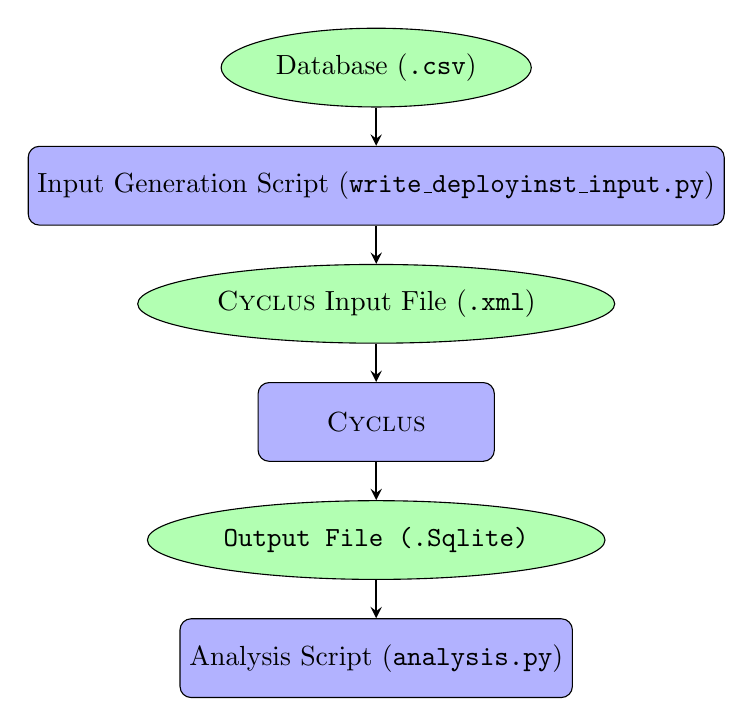
\begin{tikzpicture}[node distance=1.5cm]
\node (database) [object] {Database (\texttt{.csv})};
\node (script) [process, below of=database] {Input Generation Script (\texttt{write\_deployinst\_input.py})};
\node (input) [object, below of=script] {\Cyclus Input File (\texttt{.xml})};
\node (cyclus) [process, below of=input]{\Cyclus};
\node (output) [object, below of=cyclus]{\texttt{Output File (\texttt{.Sqlite})}};
\node (script2) [process, below of=output]{Analysis Script (\texttt{analysis.py})};

\draw [arrow] (database) -- (script); 
\draw [arrow] (script) -- (input); 
\draw [arrow] (input) -- (cyclus);
\draw [arrow] (cyclus) -- (output);
\draw [arrow] (output) -- (script2);
\end{tikzpicture}
}
\caption{Computational Workflow for this work. The green circles represent files, and the blue
         boxes represent codes that process the files.}
\label{diag:comp}
\end{figure}


Projections of future reactor deployment in this simulation are based on
assessment of analyses from references such as \gls{PRIS} for reactors planned
for construction \cite{iaea_pris_2017}, the World Nuclear Association
\cite{world_nuclear_association_nuclear_2017}, and works on the future of
nuclear power in a global \cite{joskow_future_2012} and European context
\cite{hatch_politics_2015}.  The projections extend to 2050 at the latest.  Later sections explain, in detail, the specific plans for each \gls{EU} nation.

\Cref{tab:eu_deployment} lists the reactors that are currently  planned or
under construction.  All  planned constructions are completed without delay or
failure and are assumed to reach a lifetime of 60 years.  


\begin{table}[h]
    \centering

    \label{tab:eu_deployment}
    \scalebox{0.9}{
    \begin{tabular}{ccccc}
        \hline
        \textbf{Exp. Operational }&\textbf{ Country} &\textbf{ Reactor} & \textbf{Type} & \textbf{Gross \gls{MWe}}\\
        \hline
        2018 & Slovakia  & Mochovce 3 & PWR & 440\\
        2018 & Slovakia & Mochovce 4 & PWR & 440 \\
        2018 & France & Flamanville 3 & PWR & 1600 \\
        2018 & Finland & Olkilouto 3 & PWR & 1720 \\
        2019 & Romania & Cernavoda 3 & PHWR & 720 \\
        2020 & Romania & Cernavoda 4 & PHWR & 720 \\
        2024 & Finland & Hanhikivi & VVER1200 & 1200 \\
        2024 & Hungary & Paks 5 & VVER1200 & 1200 \\
        2025 & Hungary & Paks 6 & VVER1200 & 1200 \\
        2025 & Bulgaria & Kozloduy 7 & AP1000? & 950 \\
        2026 & UK & Hinkley Point C1 & EPR & 1670 \\
        2027 & UK & Hinkley Point C2 & EPR & 1670 \\
        2029 & Poland & Choczewo & N/A & 3000 \\
        2035 & Poland & N/A & N/A & 3000 \\
        2035 & Czech Rep & Dukovany 5 & N/A & 1200 \\
        2035 & Czech Rep & Temelin 3 & AP1000 & 1200 \\
        2040 & Czech Rep & Temelin 4 & AP1000 & 1200 \\
        \hline
    \end{tabular}
    }
    \label{tab:eu_deployment}
    \caption {Power Reactors under construction and planned.
        Replicated from \cite{world_nuclear_association_nuclear_2017}.}
\end{table}
\FloatBarrier

For each \gls{EU} nation, the growth trajectory is categorized from
``Aggressive Growth'' to ``Aggressive Shutdown''. Aggressive growth is
characterized by a rigorous expansion of nuclear power while
Aggressive Shutdown is characterized as a transition to rapidly
de-nuclearize the nation's electric grid. A nation's growth trajectory is
categorized into five degrees depending on G, the growth trajectory metric.

 \[
 G = \left\{\begin{array}{ll}
 \text{Aggressive Growth}, & \text{for } G \geq 2\\
 \text{Modest Growth}, & \text{for } 1.2 \leq G < 2\\
 \text{Maintanence}, & \text{for } 0.8 \leq G < 1.2 \\
 \text{Modest Reduction}, & \text{for } 0.5 \leq G< 0.8\\
 \text{Aggressive Reduction}, & \text{for } G \leq 0.5
 \end{array}\right\} = \frac{C_{2040}}{C_{2017}}\\\\
 \]
 \[
  G = \text{Growth Trajectory  } [-] 
 \]
 \[
 C_{i} = \text{Nuclear Capacity in Year i  } [\gls{MWe}]
 \]

The growth trajectory and specific plan of each nation in the \gls{EU} 
is listed in Table \ref{tab:eu_growth}.


Figure \ref{fig:eu_pow} displays the
timeseries of installed capacity in \gls{EU} nations.


\begin{table}[h]
    \centering
        \begin{tabular}{ccc}
            \hline 
                    
                    \textbf{Nation} & \textbf{Growth Trajectory} & \textbf{Specific Plan }\\
                    \hline
                    UK & Aggressive Growth & {\small  13 units (17,900 \gls{MWe}) by 2030.}\\
                    Poland & Aggressive Growth &  {\small Additional 6,000 \gls{MWe} by 2035.}\\
                    Hungary & Aggressive Growth &  {\small Additional 2,400 \gls{MWe} by 2025.} \\ 
                    Finland & Modest Growth &  {\small Additional 2,920 \gls{MWe} by 2024.}\\
                    Slovakia & Modest Growth & {\small Additional 942 \gls{MWe} by 2025.}\\
                    Bulgaria & Modest Growth &  {\small Additional 1,000 \gls{MWe} by 2035.} \\
                    Romania & Modest Growth &  {\small Additional 1,440 \gls{MWe} by 2020.} \\
                    Czech Rep. & Modest Growth & {\small  Additional 2,400 \gls{MWe} by 2035.}\\
                    France & Modest Reduction & {\small No expansion or early shutdown.}\\
                    Slovenia & Modest Reduction & {\small No expansion or early shutdown.}\\
                    Netherlands & Modest Reduction & {\small No expansion or early shutdown.}\\
                    Lithuania & Modest Reduction & {\small No expansion or early shutdown.}\\
                    Spain & Modest Reduction &  {\small No expansion or early shutdown.} \\
                    Italy & Modest Reduction & {\small No expansion or early shutdown. }\\
                    Belgium & Aggressive Reduction & All shut down 2025.\\
                    Sweden & Aggressive Reduction & All shut down 2050.\\
                    Germany & Aggressive Reduction & All shut down by 2022.\\
                    \hline
                    
        \end{tabular}

    \caption {Future Nuclear Programs of \gls{EU} Nations \cite{world_nuclear_association_nuclear_2017}}
  \label{tab:eu_growth}
\end{table}
\FloatBarrier

\begin{figure}[htbp!]
    \begin{center}
        \includegraphics[scale=0.6]{./images/eu_future/power_plot.png}
    \end{center}
    \caption{The timeseries of installed nuclear capacity in the EU is separated by \texttt{Region}s in \Cyclus.
             The sudden drops in capacity are caused by nuclear phaseout plans by nations such as Germany and Belgium.
             The predictions into the future are made to the farthest planned future.
             }
    \label{fig:eu_pow}
\end{figure}



\subsection{French \gls{SFR} Deployment Schedule}

From 2040,
600-\gls{MWe} \glspl{SFR} are deployed to make up for the 
decommissioned \gls{LWR} capacities, to remain an installed 
capacity of 66,000 \gls{MWe}. 

\begin{figure}[htbp!]
        \begin{center}
                \includegraphics[scale=0.6]{./images/french-transition/power_plot.png}
        \end{center}
        \caption{This plot shows the potential French transition from \glspl{LWR} to \glspl{SFR}.
                 The aggressive growth of nuclear in the 1980s leads to a substantial shutdown
                 of nuclear in the 2040s, which would be replaced by new \glspl{SFR}. The net
                 capacity is kept at a constant of 66 GWe.}
        \label{fig:sfr_num}
\end{figure}
\begin{figure}[htbp!]
    \begin{center}
        \includegraphics[scale=0.6]{./images/french-transition/sfr_deploy.png}
    \end{center}
    \caption{The deployment of \glspl{SFR} in France is characterized by a period of
             aggressive building. An average of four reactors are built per year to
             make up for the decommissioned power plants built in the 1980s and 1990s.
             The second period of aggressive building occurs when the first generation
             of \glspl{SFR} decommission after 80 years.}
    \label{fig:dep}
\end{figure}

\begin{figure}[htbp!]
    \begin{center}
        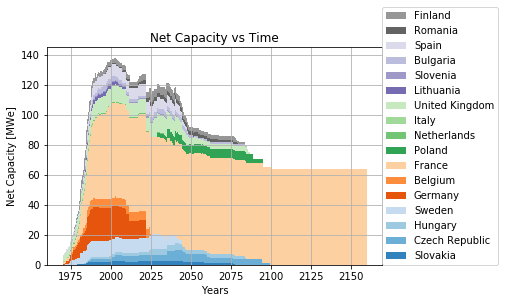
\includegraphics[scale=0.6]{./images/eu_future/onesim.png}
    \end{center}
    \caption{The total deployment scheme of the simulation. The historical
             operation \gls{EU} reactors is followed by the French
             transition to \glspl{SFR}.}
    \label{fig:tot_dep}
\end{figure}


\Cref{fig:sfr_num} and \ref{fig:dep} display
the French transition to \glspl{SFR} over time.
\Cref{fig:tot_dep} displays the total deployment
scheme of the simulation.
The steep transition from 2040 to 2060 reflects the scheduled
decommissioning of reactors built in the 1975-2000
era of aggressive nuclear growth in France.

In reality, building five reactors every year is highly unrealistic. However,
this analysis is to analyze material flow, claiming that, if such an aggressive
deployment scheme was to take place, the \glspl{SFR} would have enough fuel.
More realistically, the deployment of new \glspl{SFR} can be spread out by
staggering scheduled decommissioning of \glspl{LWR} through lifetime extensions.
An analysis of the effect of \gls{LWR} lifetime extension is shown in a later section.



\subsection{Material Flow}
A source provides natural uranium, which is enriched by an enrichment
facility to produce \gls{UOX}, while disposing enrichment waste (tails)
to the sink. The enriched \gls{UOX} fuels
the \gls{LWR}s and \gls{UOX} waste is produced. The used fuel
is sent to a pool to cool for at least 3 years \cite{carre_overview_2009}.

The cooled fuel is then reprocessed to separate plutonium and uranium,
or sent to a repository.
The plutonium mixed with depleted uranium (tails) makes \gls{MOX}.
Reprocessed uranium is unused and stockpiled. Uranium is reprocessed
in order to separate the raffinate (minor actinides and fission products)
from `usable' material. Though neglected in this paper, reprocessed
uranium may substitute depleted uranium for \gls{MOX} production. In the
simulations, sufficient depleted uranium existed that using reprocessed
uranium was overlooked. However, further in the future where the depleted
uranium inventory drains, reprocessed uranium (or, natural uranium) will need to be utilized. 

The simulated fuel cycle is illustrated in figure \ref{diag:fc}.



% Define block styles
\tikzstyle{decision} = [diamond, draw, fill=blue!20, 
text width=4.5em, text badly centered, node distance=3cm, inner sep=0pt]
\tikzstyle{block} = [rectangle, draw, fill=blue!20, 
text width=5em, text centered, rounded corners, minimum height=4em]
\tikzstyle{line} = [draw, -latex']
\tikzstyle{cloud} = [draw, ellipse,fill=red!20, node distance=3cm,
minimum height=2em]


\begin{figure}
        \centering
        \scalebox{0.6}{
                \begin{tikzpicture}[align=center, node distance = 3cm and 3cm, auto]
                % Place nodes
                \node [block] (sr) {Mine (\texttt{SOURCE})};
                \node [cloud, below of=sr] (nu) {Nat U};
                \node [block, below of=nu] (enr) {Enrichment ({\footnotesize \texttt{ENRICHMENT}})};
                \node [cloud, below of=enr] (uox) {\gls{UOX}};
                \node [block, below of=uox] (lwr) {\gls{LWR} (\texttt{REACTOR})};
                \node [cloud, right of=lwr] (snf) {\gls{UNF}};
                \node [cloud, right of=uox] (cunf) {Cooled \gls{UNF}};
                \node [block, right of=snf] (pool) {Pool (\texttt{Storage})};
                \node [cloud, left of=lwr] (tl2) {Dep U};
                \node [cloud, right of=enr] (tl) {Dep U};
                \node [block, right of=tl] (sk) {Repository (\texttt{SINK})};
                \node [cloud, below of=pool] (cunf2) {Cooled \gls{UNF}};
                \node [block, below of=snf] (rep) {{\small Reprocessing ({\footnotesize \texttt{SEPARATIONS}})}};
                \node [cloud, below of=rep] (u) {Sep. U} ;
                \node [cloud, left of=rep] (pu) {Sep. Pu};
                \node [block, left of=pu] (mix) {Fabrication (\texttt{MIXER})};
                \node [cloud, below of=mix] (mox) {\gls{MOX}};
                \node [block, below of=mox] (mxr) {\gls{MOX} Reactors};
                \node [cloud, right of= mxr] (snmox) {Spent \gls{MOX}};
                
                \draw[->, thick] (sr) -- (nu);
                \draw[->, thick] (nu) -- (enr);
                \draw[->, thick] (enr) -- (tl);
                \draw[->, thick] (enr) -- (tl2);
                \draw[->, thick] (tl) -- (sk);
                \draw[->, thick] (tl2) -- (mix);
                \draw[->, thick] (enr) -- (uox);
                \draw[->, thick] (uox) -- (lwr);
                \draw[->, thick] (lwr) -- (snf);
                
                \draw[->, thick] (lwr) -- (snf);
                \draw[->, thick] (snf) -- (pool);
                \draw[->, thick] (pool) -- (cunf);
                \draw[->, thick] (pool) -- (cunf2);
                \draw[->, thick] (cunf) -- (sk);
                \draw[->, thick] (cunf2) -- (rep);
                
                \draw[->, thick] (rep) -- (u);
                \draw[->, thick] (rep) -- (pu);
                \draw[->, thick] (pu) -- (mix);
                \draw[->, thick] (mix) -- (mox);
                \draw[->, thick] (mox) -- (mxr);
                \draw[->, thick] (mxr) -- (snmox);
                \draw[->, thick] (snmox) -- (rep);
                
                \end{tikzpicture}
        
                }
                \caption{The blue boxes represent fuel cycle facilities, and the red ovals
                         represent materials. The facility names in parenthesis are archetype names
                         used in \Cyclus. \gls{MOX} Reactors include both French \glspl{PWR} and
                         \glspl{SFR}.}
                \label{diag:fc}
\end{figure}
\FloatBarrier

\section{Scenario Specifications}

The scenario specifications  are
listed in tables \ref{tab:gen}, \ref{tab:sim_eu}, and \ref{tab:sim_france}.
The reprocessing and \gls{MOX} fabrication capacity in France
prior to 2020 is modeled after the 
French La Hague and MELOX site \cite{schneider_spent_2008, hugelmann_melox_1999}.


\begin{table}[h]
    \centering
    \begin{tabularx}{\textwidth}{bb}
        \hline
        \textbf{Specification} &\textbf{ Value} \\
        \hline
        Simulation Time & 1970-2160 \\ 
        Reprocessed Uranium Usage &  None. Stockpile reprocessed U \\
        Storage Residence Time & 36 months \\
        \gls{SFR} available year & 2040 \\
        Production of \gls{ASTRID} fuel begins & 2020 \\
        \hline
    \end{tabularx}
    \caption {General Simulation Specifications}
    \label{tab:gen}
\end{table}

\begin{table}[h]
    \centering
    \begin{tabularx}{\textwidth}{bb}
        \hline
        \textbf{Specification} &\textbf{ Value} \\
        \hline
        Reprocessing Capacity & 91.6 MTHM of \gls{UNF} per month \cite{schneider_spent_2008} \\
        Reprocessing Efficiency & 99.8\% \\
        Reprocessing Streams & plutonium and uranium \\
        \gls{MOX} Fabrication Throughput & 16.25 MTHM of \gls{MOX} per month  \cite{hugelmann_melox_1999} \\
        \gls{MOX} Fuel Reprocessing Stage &  Used \gls{MOX} is not reprocessed. \\  
        \hline
    \end{tabularx}
    \caption {Specification for Historical Operation of \gls{EU}}
    \label{tab:sim_eu}
\end{table}

\begin{table}[h]
    \centering
    \begin{tabularx}{\textwidth}{bb}
        \hline
        \textbf{Specification }& \textbf{Value} \\
        \hline
        Separation Efficiency & 99.8 \% \\
        Reprocessing Streams & plutonium and uranium \\
        \gls{ASTRID} Fuel Reprocessing Stage &  Used \gls{MOX} gets reprocessed infinitely. \\
        \hline
    \end{tabularx}
    \caption {Specification for French Transition to \glspl{ASTRID} }
    \label{tab:sim_france}
\end{table}

\pagebreak

\section{Reactor Specifications}
Three major reactors are used in the simulation, \gls{PWR}, \gls{BWR}, and ASTRID-type \gls{SFR} reactors.


For \glspl{LWR}, we used a linear core size model to capture
varying reactor capacity. For example, a 
1,200 \gls{MWe} PWR has $193*\frac{1,200}{1,000} = 232$ \gls{UOX} assemblies, each
weighing 523.4 kg.
After each 18 month cycle, one-third of the 
core (77 assemblies) discharges. Refueling
is assumed to take 2 months to complete, during which the reactor
is shut down. The specifications are defined in 
\Cref{tab:reactor-specs} details the reactor specifications in this simulation.

\begin{table}[h]
    \centering
    \begin{tabular}{cccc}
        \hline
        \textbf{Specification} & \textbf{\gls{PWR} \cite{sutharshan_ap1000tm_2011}} & \textbf{\gls{BWR} \cite{hinds_next-generation_2006}} & \textbf{\gls{SFR}} \cite{varaine_pre-conceptual_2012}\\
        \hline
                Lifetime [y] \tablefootnote{The simulated reactor lifetime reaches the licensed lifetime unless 
        the reactor is shut down prematurely.} & 60 & 60 & 80 \\
                Cycle Time [mos.]& 18 & 18 & 12\\ 
                Refueling Outage [mos.]& 2 & 2  & 2\\
                Rated Power [\gls{MWe}] & 1000 & 1000 & 600\\
                Assembly mass [kg] & 523.4 & 180 & -- \\
                Batch mass [kg] & -- & -- & 5,568\\
                Discharge Burnup [GWd/tHM] & 51 & 51 & 105 \\
                Assemblies per core \tablefootnote{Number of assemblies and corresponding \gls{LWR} core 
        masses are reported for a 1000-\gls{MWe} core. Reactors with different core  
        powers are modeled with a linear mass assumption.} & 193  & 764 & -- \\

                Batches per core & 3 & 3 & 4\\
                Initial Fissile Loading & 3.1 t  $^{235}U$ & 4.2 t  $^{235}U$ & 4.9 t  Pu \\
                Fuel & \gls{UOX} or \gls{MOX} & \gls{UOX} & \gls{MOX} \\
        \hline
    \end{tabular}
        \caption {Model \gls{LWR} and \gls{ASTRID} specifications used for the simulations are listed, and \glspl{LWR} are modified
        linearly for varying power capacity. }
    \label{tab:reactor-specs}

    \end{table}


\subsection{Material Definitions}
Depletion calculations of the nuclear fuel are recipe-based, such that a fresh 
and used fuel recipe is defined for each reactor type.
For the compositions of the used fuel, a reference depletion calculation
from ORIGEN is used (see \cref{tab:comp}). The recipe has also been used for
\cite{wilson_adoption_2009}.

\begin{table}[h]
    \centering
%   \scalebox{0.86}{
        \begin{tabular}{cccc}
            \hline
             & \multicolumn{3}{c}{ Composition [\%]} \\
            Recipe & U-235  & U-238  & Pu \\ 
            \hline
            Fresh \gls{UOX} Fuel & 3.1 & 96.9 & -   \\ 
            Fresh \gls{MOX} Fuel & 0.2 & 90.7 & 9.1 \\ 
            Fresh \gls{ASTRID} Fuel & 0.2 & 77.7 & 22 \\
            \hline
        \end{tabular}
        \caption{Fresh fuel compositions used for the simulation \cite{wilson_adoption_2009, varaine_pre-conceptual_2012}.}
        \label{tab:sim_result}
\end {table}

\section{Results}

\subsection{Nuclear Material Inventory}

\Cref{tab:sim_result1} lists \gls{EU} material inventory in 2050.

\begin{table}[h]
	\centering
%	\scalebox{0.86}{
		\begin{tabular}{cccc}
			\hline
			\textbf{Category } & \textbf{Value} & \textbf{Unit} & \textbf{Specifics}\\ \hline
			UOX Usage  & 158,794 & MTHM &  \\ 
			MOX Usage  & 6,671 & MTHM & \\ 
			\textbf{Used UOX Stored}  & \textbf{95,161} & MTHM & \gls{UNF} that is not reprocessed\\
			\textbf{Used UOX Stored (France)} & \textbf{9,979} & MTHM & \gls{UNF} that is not reprocessed \\
			Tails  & 979,463 & MTHM & \\ 
			Natural U Used  & 1,141,916 & MTHM & \\ \hline
		\end{tabular}
		\caption{Nuclear material inventory in the \gls{EU} in 2050 is summarized. 
				 The difference between total \gls{UOX} usage and \gls{UOX} stored is the amount
				 that has been reprocessed for \gls{MOX}. Only the stored \gls{UOX} is used for \gls{ASTRID} fuel production.}
		\label{tab:sim_result1}
\end {table}
\FloatBarrier


Figures \ref{fig:eu_tail} and \ref{fig:eu_snf} show the 
accumulation of tails and used fuel over time in \gls{EU}.
Tails accumulate as a by-product of uranium enrichment. For every
ton of \gls{UOX} fuel, about nine times of tails is produced. 
Spent fuel is discharged from reactors every refueling period.
The entire core is discharged when the reactor decommissions.
A total of about $1,000,000 MTHM$ of tails and $100,000 MTHM$ of
\gls{UNF} accumulate in 2050.
Figure \ref{fig:eu_fuel} shows the amount of fuel used in \gls{EU}.


\begin{figure}[htbp!]
	\begin{center}
		\includegraphics[scale=0.7]{./images/eu_future/tails.png}
	\end{center}
	\caption{This plot shows the timeseries of tails mass accumulation and discharge in the \gls{EU} nations.
			 Tails mass accumulation is fairly steady, with peaks occurring when
			 new reactors are deployed.}
	\label{fig:eu_tail}
\end{figure}

\begin{figure}[htbp!]
	\begin{center}
		\includegraphics[scale=0.7]{./images/eu_future/total_fuel.png}
	\end{center}
	\caption{This plot shows the timeseries of total fuel usage in the \gls{EU} nations.}
	\label{fig:eu_fuel}
\end{figure}


\begin{figure}[htbp!]
	\begin{center}
			\includegraphics[scale=0.7]{./images/eu_future/snf_discharge.png}
	\end{center}
	\caption{This plot displays the timeseries of \gls{UNF} accumulation and discharge in the \gls{EU} nations.
			 The peaks are caused by decommissioning of reactors, where all the core is sent to the repository.}
	\label{fig:eu_snf}
\end{figure}
\FloatBarrier


\begin{table}[h]
	\centering
	\begin{tabular}{ccc}
		\hline
		\textbf{Isotope} & \textbf{Mass Fraction in Used Fuel [\%]} & \textbf{Quantity [t]} \\ \hline
		Pu238 & 0.0111 & 10.5628 \\ 
		Pu239 & 0.518 & 492.93 \\ 
		Pu240 & 0.232 & 220.7 \\ 
		Pu241 & 0.126 & 119.9 \\ 
		Pu242 & 0.0487 & 46.3 \\ \hline
		\textbf{Total} & \textbf{0.9358} & \textbf{890.5} \\ \hline
	\end{tabular}
	\caption{Plutonium From \gls{UNF} Inventory. This table assumes no decay
			 took place. The long half-life of the fissile Pu-239 (24,100 years)
			 weakens the impact of decay on the usability of \gls{UNF}.}
	\label{tab:pu}
\end{table}


\Cref{tab:pu} lists the isotope, mass fraction,
and quantity of plutonium that can be obtained from the 2050 \gls{UNF} inventory.


\subsection{French \gls{SFR} Deployment}

Reprocessing \gls{UNF} collected from all EU nations can start approximately
180 \glspl{SFR}. With the \gls{SFR} breeding ratio of over one, France can transition into
a fully \gls{SFR} fleet without extra construction of \glspl{LWR}. 

From Varaine et al. \cite{varaine_pre-conceptual_2012}, a French
ASTRID-type \gls{SFR} of capacity 600 \gls{MWe} needs $1.225$ tons of
plutonium a year, with an initial plutonium loading of $4.9$ tons. 
Thus, the number of \glspl{SFR} that can be loaded with the reprocessed
plutonium from \gls{UNF} can be estimated to $\frac{Pu \ from \ legacy \ \gls{UNF}}{4.9} \approx 181$ \glspl{SFR},
assuming infinite reprocessing and fabrication capacity as well as
abundant depleted uranium supply. 

Also, assuming that \gls{MOX} can be recycled indefinitely,
used \gls{MOX} from an ASTRID reactor contains enough plutonium to produce a \gls{MOX} fuel with
the same mass, if mixed with depleted uranium. For example,
used \gls{MOX} from an ASTRID reactor is assumed to be 23.95\% plutonium
in this simulation (see \cref{tab:comp}), whereas a fresh \gls{MOX} is 22\% plutonium.
Separating plutonium from used \gls{MOX} from
an ASTRID reactor can create \gls{MOX} of the mass of used \gls{MOX}.
The plutonium breeding ratio in this simulation is thus assumed to be
$\approx 1.08$.

\Cref{fig:fuel} shows \gls{MOX} loaded in the \glspl{SFR} per month.
The spikes are due to initial fuel demand for new deployment of \glspl{SFR}.
The initial loading of new \glspl{SFR} are done with the \gls{MOX} created
from legacy \gls{UNF}. Once the deployed \glspl{SFR} create enough amounts
 of extra plutonium, the legacy \gls{UNF} is no longer used. 

\begin{figure}[htbp!]
	\begin{center}
		\includegraphics[scale=0.7]{./images/french-transition/where_fuel.png}
	\end{center}
	\caption{This plot shows the timeseries of fuel loaded into \glspl{SFR}.
			 The plot has peaks during a period of aggressive deployment of \glspl{SFR}
			 followed by an equilibrium at 150 \gls{MTHM}. The peaks reoccur with the
			 deployment of the second generation of \glspl{SFR}.}
	\label{fig:fuel}
\end{figure}
 \Cref{fig:pu_no_cum} shows the separated plutonium discharge
per month from the reprocessing plant. The plutonium outflux
does not precisely follow the fuel demand because \Cyclus agents have
material buffers that store commodity fuel for later usage. The reprocessed
plutonium from legacy \gls{UNF} is stored for the initial loading of \glspl{SFR}.
\Cref{tab:sfr_sim_result} lists metrics obtained from the second simulation.

\begin{figure}[htbp!]
	\begin{center}
		\includegraphics[scale=0.7]{./images/french-transition/pu.png}
	\end{center}
	\caption{This plot shows the separated plutonium discharge from the reprocessing plant.
			 The reprocessing demand for the first aggressive deployment of \glspl{SFR}
			 are lessened because the plutonium demand is met with plutonium separated from legacy \gls{UNF}.
			 The plutonium from reprocessing legacy fuel is a flat rectangle because the 
			 reprocessing throughput was set to 20 $\frac{tons}{month}$ to avoid reprocessing
			 all the legacy in one timestep. }
	\label{fig:pu_no_cum}
\end{figure}

\begin{table}[h]
	\centering
	\scalebox{0.86}{
		\begin{tabular}{ccc}
			\hline
			\textbf{Category} & \textbf{Unit} & \textbf{Value}  \\ \hline
			Total MOX used & MTHM & 63,820  \\ 
			\textbf{Average UOX Reprocessing} & MTHM/month & \textbf{118.92} \\
			\textbf{Average Total Reprocessing} & MTHM/month & \textbf{73.27} \\
			\textbf{Average Fuel Fabrication} & MTHM/month & \textbf{45.2} \\
			Total \glspl{SFR} Deployed & & 220 \\ 
			Total Plutonium Reprocessed & MTHM & 15,099 \\ 
			Total \gls{ASTRID} fuel from UOX Waste & MTHM & 2,923  \\ 
			Total \gls{ASTRID} fuel from MOX Waste & MTHM  & 60,535 \\ 
			Total Tails used & MTHM & 49,779 \\ 
			\textbf{Total legacy UNF reprocessed} & MTHM & \textbf{54,111} \\ 
			Total Reprocessed Uranium Stockpile & MTHM & 183,740 \\ 
			Total Raffinate & MTHM & 33,806 \\ \hline
		\end{tabular}}
		\caption {Listed are the metrics from the French transition to \gls{SFR} scenario.
				  The total legacy \gls{UNF} reprocessed is the amount of \gls{UNF} France would need
				  for a transition into a fully \gls{SFR} fleet. The tails used is around ninth
				  of the original tails inventory from the previous simulation.}
		\label{tab:sfr_sim_result}
\end {table}

Despite the large amount of initial plutonium that has to be reprocessed
prior to \gls{ASTRID} deployment, the 20 years of preparation of
\gls{ASTRID} fuel (2020-2040) allows a reasonable level of average
\gls{UOX} reprocessing capacity demand. \gls{UOX} reprocessing continues 
until 2057, when the \gls{ASTRID} spent fuel can supply the plutonium
for its own fuel.



\section{Sensitivity Analysis}

An important aspect of any fuel cycle transition scenario
is the accrual of fissile materials for new reactor deployment.
The collaborative strategy makes a transition possible 
from the perspective of material availability,
but the aggressive transition demands a significant increase in reprocessing capacity.

We explored the impact of two key variables, the lifetime of French \glspl{LWR} and the
breeding ratio of \gls{ASTRID} reactors. The range over which we varied these parameters (table \ref{tab:sen_par})
sought to capture the full span of their uncertainty.

Note that \gls{ASTRID} breeding ratios are arbitrarily increased
by direct adjustment of their output fuel compositions. We did not 
take into account the other reactor parameters (e.g. core size, initial
fuel composition, fuel residence time, etc.)
that would be neccessary to achieve a higher breeding ratio. More detailed analyses
of the reactor physics and their effect on this transition scenario 
should be pursued in future work.


\begin{table}[h]
    \centering
    \caption{Both \gls{LWR} lifetime and \gls{ASTRID} breeding ratio impact 
    transitional reprocessing demand.}
    \begin{tabularx}{\textwidth}{lrr}
        \hline
        \textbf{Parameter} & \textbf{Default} & \textbf{Values} \\
        \hline
        Breeding Ratio of \glspl{ASTRID} & 1.08 & 1.11, 1.15, 1.18 \\ 
        Lifetime of French \glspl{LWR} [years] & 60  & 65, 70, 80 \\
        \hline
    \end{tabularx}
    \label{tab:sen_par}
\end{table}

\subsection{Breeding Ratio}


Increase in the breeding ratio of \gls{ASTRID} reactors
decreases the total reprocessing demand, as shown in 
figure \ref{fig:br_rep}.
The demand previous to 2050 is unaffected by the 
breeding ratio because only \gls{UOX} \gls{UNF} is reprocessed.

\begin{figure}[htbp!]
    \begin{center}
        \includegraphics[scale=0.6]{./images/sensitivity/br_tot_rep.png}
    \end{center}
    \caption{Increasing the breeding ratio decreases the monthly reprocessing 
    demand.}
    \label{fig:br_rep}
\end{figure}

The sensitivity analysis also shows, as demonstrated in figure \ref{fig:br_uox} that 
increasing the breeding ratio decreases the mass of \gls{UOX} \gls{UNF} 
required for the transition. The \glspl{ASTRID} produce 
more plutonium, reducing the plutonium demand from 
reprocessed \gls{UOX}. However, since \gls{LWR} \gls{UNF} is not
the limiting factor, increasing the breeding ratio does not play a significant
role in the transition scenario, especially considering the technical difficulty
in achieving a high breeding ratio.

\begin{figure}[htbp!]
    \begin{center}
        \includegraphics[scale=0.6]{./images/sensitivity/br_uox_unf_cum.png}
    \end{center}
    \caption{Sensitivity analysis demonstrates that increasing the breeding 
    ratio decreases the required \gls{UOX} \gls{UNF}. }
    \label{fig:br_uox}
\end{figure}

The differential impacts of varying the breeding ratios are
shown in table \ref{tab:br_diff}. The difference were calculated
using the following equation:

\[ \epsilon = \frac{(x - x_{base})}{x_base} * 100 \]

\begin{table}[h]
	\centering
	\caption{Percent difference of total \gls{LWR} \gls{UNF} reprocessed
		for transition and total reprocessing demand for the simulation.}
	\begin{tabular}{lrrrr}
		\hline
		\multirow{2}{*}{\textbf{Parameter}} & \multicolumn{4}{c}{\% Difference} \\
		 & \textbf{1.08}& \textbf{1.11} & \textbf{1.15} & \textbf{1.18} \\
		\hline
		Total reprocessing demand & 0.0 & -1.8 & -2.6 & -3.4 \\ 
		\gls{LWR} \gls{UNF} reprocessed & 0.0  & -4.9 & -8.0 & -9.7 \\
		\hline
	\end{tabular}
	\label{tab:br_diff}
\end{table}


\subsection{Lifetime Extension of French \glspl{LWR}}\label{sec:life}
Extending the lifetime of French \glspl{LWR} lowers the average
monthly \gls{UOX} reprocessing demand, since the \gls{ASTRID} deployment becomes 
delayed (shown in figure \ref{fig:pow_diff}). The plutonium demand is delayed,
 allowing the reprocessing plant more time to prepare plutonium for \gls{ASTRID} reactors.

\begin{figure}[htbp!]
    \begin{center}
        \includegraphics[scale=0.7]{./images/sensitivity/pow_ratio.png}
    \end{center}
    \caption{The ratio of \glspl{ASTRID} to \glspl{LWR} in France demarcates 
    the transition period.}
    \label{fig:pow_diff}
\end{figure}

Figure \ref{fig:ext_uox} shows the decrease in the average monthly
\gls{UOX} reprocessing burden with increased \gls{LWR} lifetimes.
This is balanced by extending the necessary duration of 
\gls{LWR} \gls{UNF} reprocessing,
so
the total amount of \gls{LWR} \gls{UNF} reprocessed (shown in table
\ref{tab:ext_diff}).


\begin{figure}[htbp!]
	\begin{center}
		\includegraphics[scale=0.7]{./images/sensitivity/ext_uox_rep.png}
	\end{center}
	\caption{Increasing the lifetime of French \glspl{LWR} decreases the monthly
		\gls{UOX} reprocessing demand, but increases the duration of \gls{LWR} \gls{UNF}
		reprocessing, thereby increasing the total amount of \gls{LWR} \gls{UNF} reprocessed.}
	\label{fig:ext_uox}
\end{figure}

Figure \ref{fig:ext_all} shows that lifetime extension has little
effect on the average total monthly reprocessing demand, because
the amount of plutonium in the \gls{ASTRID} used fuel remains the same.
The delay of \gls{ASTRID} deployment simply provides more time for
France to prepare the fuel. 
The longer lifetimes of \glspl{LWR} delay transition, and gives France
time to accumulate \gls{LWR} \gls{UNF}. However, it does not reduce
the total reprocessing capacity required for transition.



\begin{figure}[htbp!]
    \begin{center}
        \includegraphics[scale=0.7]{./images/sensitivity/ext_tot_rep.png}
    \end{center}
    \caption{Increasing the lifetime of French \glspl{LWR} simply delays the
             reprocessing demand, and has little impact on the total 
     reprocessing capacity required.}
    \label{fig:ext_all}
\end{figure}

\begin{table}[h]
	\centering
	\caption{Percent difference of total \gls{LWR} \gls{UNF} reprocessed
		for transition and total reprocessing demand for the simulation.}
	\begin{tabular}{lrrrr}
		\hline
		\multirow{2}{*}{\textbf{Parameter}} & \multicolumn{4}{c}{\% Difference} \\
		& \textbf{base}& \textbf{5 years} & \textbf{10 years} & \textbf{20 years} \\
		\hline
		Total reprocessing demand & 0.0 & -5.9 & -3.3 & 3.1 \\
		\gls{LWR} \gls{UNF} reprocessed & 0.0  & 4.2 & 8.6 & 17.8 \\
		\hline
	\end{tabular}
	\label{tab:ext_diff}
\end{table}


\FloatBarrier
\section{Conclusion}

This work demonstrates that France can transition into
a fully \gls{SFR} fleet with installed capacity of 66,000 \gls{MWe} without
building additional \glspl{LWR}
if France receives \gls{UNF} from other \gls{EU} nations.
Supporting the \gls{SFR} fleet requires an average 
reprocessing capacity of 63.23 \gls{MTHM} per month,
and an average fabrication capacity of 45.32 \gls{MTHM} per month.

The sensitivity study explored the effect of increased \gls{SFR} breeding
ratio and existing \gls{LWR} lifetime extension. Increasing the breeding
ratio reduced the amount of \gls{LWR} \gls{UNF} required to transition
up to $9.7\%$ and decreased the total reprocessing demand up to $3.4\%$.
Increasing the lifetime of existing \glspl{LWR} was not significant
in reducing reprocessing demand, but provided the benefit of delayed
transition.

Since most \gls{EU} nations do not have an operating \gls{UNF}
repository or a management plan, they have a strong incentive
to send their \gls{UNF} to France. In particular, the nations
planning aggressive nuclear reduction will be able phase out nuclear
without constructing a permanent repository. France has an
incentive to take this fuel, since recycling used fuel from
other nations will allow France to meet their MOX demand
without new construction of \glspl{LWR}.

Table \ref{tab:which_send} lists \gls{EU} nations and their \gls{UNF} inventory
in 2050. We analyzed a strategy in which 
the nations reducing their nuclear fleet send their \gls{UNF} to France.
The sum of \gls{UNF} from Italy, Slovenia, Belgium, Spain and Germany
provides enough \gls{UNF} for the simulated transition ($\approx 53,000$ MTHM). 
These nations are shown in bold in table \ref{tab:which_send}.
Sweden is not considered because of its concrete waste management plan.

If France receives \gls{LWR} \gls{UNF} from all \gls{EU} nations,
except Sweden and Finland,
it will have a surplus of $30,648$ MTHM of \gls{LWR} \gls{UNF}. This
inventory can be leveraged to increase nuclear power capacity as
the transition takes place. However, pragmatic limitations such
as new reactor construction, reprocessing throughput, and
political concerns remain.

\begin{table}[h]
    \centering
    \caption {\gls{EU} nations and their respective \gls{UNF} inventory.} 
                \begin{tabularx}{\textwidth}{llr}
                    \hline 
                    \textbf{Nation} & \textbf{Growth Trajectory} & \small{\textbf{UNF in 2050 [MTHM] }}\\
                    \hline
                    Poland & Aggressive Growth & 1,807\\
                    Hungary & Aggressive Growth & 3,119 \\ 
                    UK & Aggressive Growth & 13,268\\
                    Slovakia & Modest Growth & 2,746\\
                    Bulgaria & Modest Growth & 3,237 \\
                    Czech Rep. & Modest Growth & 4,413\\
                    Finland & Modest Growth &  5,713\\
                    Netherlands & Modest Reduction & 539\\
                    \textbf{Italy} & \textbf{Modest Reduction} & \textbf{583}\\
                    \textbf{Slovenia} & \textbf{Modest Reduction} & \textbf{765}\\\
                    Lithuania & Modest Reduction & 2,644 \\
                    \textbf{Belgium} & \textbf{Aggressive Reduction} & \textbf{6,644}\\
                    \textbf{Spain} & \textbf{Modest Reduction} &  \textbf{9,771} \\
                    \textbf{France} & \textbf{Modest Reduction} & \textbf{12,494} \\
                    Sweden & Aggressive Reduction & 16,035\\
                    \textbf{Germany} & \textbf{Aggressive Reduction} & \textbf{23,868}\\
                    \hline
                \end{tabularx}
    
    \label{tab:which_send}

\end{table}

On the other hand, in these simulations, some complex political and economic factors were not incorporated and various assumptions were present in this scenario. For
example, Germany's current policy is to not reprocess its \gls{LWR} fuel
\cite{topfer_germanys_2011}, and this policy would create a shortage
in the supply of \gls{LWR} \gls{UNF} for \gls{ASTRID} \gls{MOX} production.
Continuation of that German policy would not, however, be incompatible
with a change in \gls{EU} policy that frees \gls{EU} countries from
creating their high level waste repositories, since France could still
agree to take in Germany's \gls{UNF} for direct disposal. The analysis
method described herein could readily be adapted to account for such possibilities. 
The collaborative option explored here may hold value for the \gls{EU} nuclear community,
and may enable France to advance more rapidly into a closed fuel cycle. 
\FloatBarrier


\section{Future Work}

Numerous assumptions for reactor physics and depletion
have been made for this work. Future work includes implementation of
a more physics-based depletion model for reactors that
can take into account the plutonium vector changes in  \gls{ASTRID} and \gls{MOX} \gls{PWR} cores.
Also, improvements can be made on incorporating enrichment differences in the initial core
batches as well as depletion variations in the end-of-life cores.

\bibliographystyle{unsrtnat}
\bibliography{bibliography}
\pagebreak
\section{Fresh and Used Fuel Composition}
\begin{table}[h]
	\centering
	\scalebox{0.75}{
		\begin{tabular}{|c|c|c|c|c|c|c|}
		\hline
		 Isotope 	 & 	Fresh UOX Fuel & 	Spent UOX Fuel (BU: $51\frac{GWdth}{MTHM}$) & Fresh SFR Fuel & Spent SFR Fuel \\ \hline 
		 He4	 & 	 	& 	9.474E-07 & 	 	 & 	7.827E-06 \\ \hline 
		 Ra226	 & 	 	& 	9.788E-14 & 	 	 & 	5.151E-14 \\ \hline 
		 Ra228	 & 	 	& 	2.750E-20 & 	 	 & 	4.904E-21 \\ \hline 
		 Pb206	 & 	 	& 	5.574E-18 & 	 	 & 	1.210E-18 \\ \hline 
		 Pb207	 & 	 	& 	1.685E-15 & 	 	 & 	1.892E-16 \\ \hline 
		 Pb208	 & 	 	& 	3.688E-12 & 	 	 & 	5.875E-11 \\ \hline 
		 Pb210	 & 	 	& 	3.023E-19 & 	 	 & 	8.143E-18 \\ \hline 
		 Th228	 & 	 	& 	8.475E-12 & 	 	 & 	1.004E-10 \\ \hline 
		 Th229	 & 	 	& 	2.727E-12 & 	 	 & 	4.065E-12 \\ \hline 
		 Th230	 & 	 	& 	2.625E-09 & 	 	 & 	2.139E-09 \\ \hline 
		 Th232	 & 	 	& 	4.174E-10 & 	 	 & 	4.425E-11 \\ \hline 
		 Bi209	 & 	 	& 	6.607E-16 & 	 	 & 	2.600E-14 \\ \hline 
		 Ac227	 & 	 	& 	3.096E-14 & 	 	 & 	4.840E-15 \\ \hline 
		 Pa231	 & 	 	& 	9.246E-10 & 	 	 & 	1.300E-10 \\ \hline 
		 U232	 & 	 	& 	0.000 & 	 	 & 	0.000 \\ \hline 
		 U233	 & 	 	& 	2.213E-09 & 	 	 & 	5.528E-09 \\ \hline 
		 U234	 & 	0.000& 	0.000 & 	 	 & 	0.000 \\ \hline 
		 U235	 & 	0.032& 	0.007 & 	0.002 & 	0.000 \\ \hline 
		 U236	 & 	 	& 	0.005 & 	 	 & 	0.000 \\ \hline 
		 U238	 & 	0.968& 	0.920 & 	0.887 & 	0.808 \\ \hline 
		 Np237	 & 	 	& 	0.000 & 	 	 & 	0.000 \\ \hline 
		 Pu238	 & 	 	& 	0.000 & 	0.001 & 	0.001 \\ \hline 
		 Pu239	 & 	 	& 	0.006 & 	0.060 & 	0.085 \\ \hline 
		 Pu240	 & 	 	& 	0.002 & 	0.027 & 	0.027 \\ \hline 
		 Pu241	 & 	 	& 	0.001 & 	0.014 & 	0.003 \\ \hline 
		 Pu242	 & 	 	& 	0.000 & 	0.005 & 	0.001 \\ \hline 
		 Pu244	 & 	 	& 	2.864E-08 & 1.508E-07 & 	5.461E-09 \\ \hline 
		 Am241	 & 	 	& 	6.442E-05 & 	 	 & 	0.001 \\ \hline 
		 Am242m	 & 	 	& 	8.533E-07 & 	 	 & 	7.961E-05 \\ \hline 
		 Am243	 & 	 	& 	0.000 & 	 	 & 	0.000 \\ \hline 
		 Cm242	 & 	 	& 	2.589E-05 & 	 	 & 	5.331E-05 \\ \hline 
		 Cm243	 & 	 	& 	0.000 & 	 	 & 	3.242E-06 \\ \hline 
		 Cm244	 & 	 	& 	8.561E-05 & 	 	 & 	0.000 \\ \hline 
		 Cm245	 & 	 	& 	5.721E-06 & 	 	 & 	3.936E-05 \\ \hline 
		 Cm246	 & 	 	& 	7.295E-07 & 	 	 & 	1.434E-05 \\ \hline 
		 Cm247	 & 	 	& 	0.000 & 	 	 & 	5.317E-07 \\ \hline 
		 Cm248	 & 	 	& 	7.691E-10 & 	 	 & 	0.000 \\ \hline 
		 Cm250	 & 	 	& 	4.280E-18 & 	 	 & 	6.407E-15 \\ \hline 
		 Cf249	 & 	 	& 	1.649E-12 & 	 	 & 	6.446E-10 \\ \hline 
		 Cf250	 & 	 	& 	2.041E-12 & 	 	 & 	6.703E-11 \\ \hline 
		 Cf251	 & 	 	& 	9.865E-13 & 	 	 & 	1.903E-12 \\ \hline 
		 Cf 252	 & 	 	& 	6.579E-13 & 	 	 & 	4.014E-14 \\ \hline 
		 H3	 & 	 	& 	8.584E-08 & 	 	 & 	1.747E-07 \\ \hline 
		 C14	 & 	 	& 	4.057E-11 & 	 	 & 	 	 \\ \hline 
		 C Other	 & 	 	& 	 	 & 	 	 & 	 	 \\ \hline 
		 Kr81	 & 	 	& 	4.216E-11 & 	 	 & 	8.038E-12 \\ \hline 
		 Kr85	 & 	 	& 	3.444E-05 & 	 	 & 	2.950E-05 \\ \hline 
		 Kr Other	 & 	 	& 	0.000 & 	 	 & 	0.000 \\ \hline 
		 Sr90	 & 	 	& 	0.001 & 	 	 & 	0.001 \\ \hline 
		 Sr Other	 & 	 	& 	0.000 & 	 	 & 	0.000 \\ \hline 
		 Tc99	 & 	 	& 	0.000 & 	 	 & 	5.391E-05 \\ \hline 
		 Tc Other	 & 	 	& 	0.000 & 	 	 & 	0.002 \\ \hline 

		\end{tabular}}
		\caption{Fresh and Spent Fuel Compositions}
		\label{tab:comp}
\end {table}




\end{document}
\grid
